\chapter{نظرية هوكل والأنظمة المترافقة}\label{ch:b2:huckel}

أضف الهيدروجين إلى الهكسين الحلقي ينطلق \qty{119}{kJ} لكل مول. والبنزين،
بروابطه الثلاث المزدوجة في حلقة من ستة كربونات، كان ينبغي أن يطلق ثلاثة أضعاف
ذلك في طريقه إلى الهكسان الحلقي؛ لكنه يطلق أقل بمقدار \qty{150}{kJ}. وتلك الطاقة
المفقودة هي استقرار الحلقة \omterm{def:b2:huckel:aromatic}{العطرية}، وهي سبب مقاومة البنزين
للإضافات التي تخضع لها الألكينات. وفي سنة 1931 حسبها إريش هوكل بمحدِّد،
بعد أن اختزل الجزيء إلى إلكتروناته $\pi$
وجيرانها. وطريقته تقريبية، لكنها تفسر لماذا تتميز الحلقات ذات الإلكترونات $\pi$ الستة،
ولماذا تمتص السلاسل المترافقة الطويلة الضوء المرئي، 
وأين يحمل الجزيء المترافق شحناته.

\begin{recall}
\Cref{ch:b2:diatomic-mos}: \omterm{def:b2:diatomic-mos:integrals}{تكامل كولوم} $\alpha$، \omterm{def:b2:diatomic-mos:integrals}{وتكامل الرنين} $\beta$،
\omterm{def:b2:diatomic-mos:integrals}{والمحدد القرني}. و\cref{ch:b2:fragment-orbitals}: مدارات $\pi$ للإيثين 
والأليل. ومجلد السنة الأولى: الأنظمة المترافقة، والرنين، والكروموفورات 
وقمم الامتصاص.
\end{recall}

\section{طريقة هوكل}

في جزيء مترافق مستوٍ، تكون مدارات $\sigma$ متناظرة ومدارات p
العمودية على المستوي ضد متناظرة بالنسبة إلى ذلك المستوي: فهي
لا تمتزج (\cref{prop:b2:diatomic-mos:symmetry})، ويمكن معالجة إلكترونات $\pi$
وحدها.

\begin{definition}[طريقة هوكل]\label{def:b2:huckel:method}
\emph{طريقة هوكل}\index{طريقة هوكل} تحسب مدارات $\pi$ لنظام
مترافق مستوٍ على أنها تراكيب $\psi = \sum_r c_r p_r$ من مدار p واحد لكل
ذرة، مع التقريبات الآتية: التداخلات $S_{rs} = 0$ من أجل $r \neq s$ (و1 من أجل $r =
s$)؛ \omterm{def:b2:diatomic-mos:integrals}{وتكاملات كولوم} كلها مساوية $\alpha$؛ \omterm{def:b2:diatomic-mos:integrals}{وتكاملات الرنين} مساوية $\beta < 0$
بين الجيران المترابطين ومعدومة فيما عدا ذلك.
\end{definition}

مع $x = (\alpha - E)/\beta$، تصير المعادلات القرنية، من أجل كل ذرة $r$،
$xc_r + \sum_{s \text{ مجاورة للذرة } r} c_s = 0$، وتكون الطاقات جذور
محدد فيه $x$ على القطر و1 بين الذرات المترابطة. وبعبارة مكافئة، $E =
\alpha + m\beta$ حيث $m$ هي القيم الذاتية لمصفوفة التجاور للهيكل
الكربوني للجزيء؛ وبما أن $\beta < 0$، فإن $m$ الموجبة توافق مستوى رابطًا.

\begin{method}[حساب هوكل]\label{met:b2:huckel:huckel}
\begin{enumerate}
  \item رقّم الذرات المترافقة؛ واكتب المصفوفة التي فيها 0 على القطر و1
        لكل زوج مترابط.
  \item أوجد قيمها الذاتية $m_k$ (بالصيغ المغلقة أدناه، أو عدديًا): $E_k =
        \alpha + m_k\beta$.
  \item املأ المستويات بدءًا من أشدها ربطًا، بإلكترونين في كل منها:
        $E_\pi = \sum_k n_k E_k$.
  \item من المعاملات المنظَّمة، احسب الشحنات ومؤشرات الروابط.
\end{enumerate}
\end{method}

\begin{proposition}[الأثر]\label{prop:b2:huckel:trace}
مجموع طاقات المدارات في نظام هوكل، وعددها $n$ وكلها مدارات $\pi$، يساوي $n\alpha$.
\end{proposition}

\begin{proof}
مجموع القيم الذاتية لمصفوفة هو أثرها؛ ومصفوفة هوكل فيها $\alpha$
في كل عنصر من عناصرها القطرية، وعددها $n$.
\end{proof}

\section{البوليينات الخطية}

\begin{theorem}[مستويات سلسلة خطية]\label{thm:b2:huckel:polyene}
لسلسلة مترافقة خطية من $n$ ذرة المستويات والمعاملات
\[
  E_k = \alpha + 2\beta\cos\frac{k\pi}{n + 1}, \qquad
  c_{jk} = \sqrt{\frac{2}{n + 1}}\,\sin\frac{jk\pi}{n + 1}, \qquad k = 1, \dots, n .
\]
\end{theorem}

\begin{proof}
المعادلات القرنية هي $c_{j-1} + xc_j + c_{j+1} = 0$ من أجل $j = 1, \dots, n$، مع
$c_0 = c_{n+1} = 0$. لنجرّب $c_j = \sin j\theta$: $\sin(j - 1)\theta + \sin(j + 1)\theta = 2\sin
j\theta\cos\theta$، فتتحقق المعادلات مع $x = -2\cos\theta$، ويتحقق $c_0 = 0$
تلقائيًا. والشرط الطرفي $c_{n+1} = \sin(n + 1)\theta = 0$ يعطي $\theta =
k\pi/(n + 1)$. ومن ثم $E = \alpha - x\beta = \alpha + 2\beta\cos\theta$. ويستعمل التنظيم
$\sum_{j=1}^n\sin^2 j\theta = (n + 1)/2$.
\end{proof}

\begin{example}[البوتاديين]\label{ex:b2:huckel:butadiene}
من أجل $n = 4$: $E = \alpha \pm 1.618\beta$، $\alpha \pm 0.618\beta$. تملأ إلكترونات $\pi$ الأربعة المستويين
الرابطين: $E_\pi = 4\alpha + 2(1.618 + 0.618)\beta = 4\alpha + 4.472\beta$. ومعاملات أدنى
مدار 0.372 و0.602 و0.602 و0.372، ومعاملات المدار التالي 0.602 و0.372 
و$-0.372$ و$-0.602$.
\end{example}

\begin{omfigure}
\begin{tikzpicture}[font=\small]
  \foreach \k/\a/\b/\c/\d/\lab in {1/0.372/0.602/0.602/0.372/{$\psi_1$, $\alpha + 1.618\beta$},
      2/0.602/0.372/-0.372/-0.602/{$\psi_2$, $\alpha + 0.618\beta$},
      3/0.602/-0.372/-0.372/0.602/{$\psi_3$, $\alpha - 0.618\beta$},
      4/0.372/-0.602/0.602/-0.372/{$\psi_4$, $\alpha - 1.618\beta$}} {
    \begin{scope}[yshift={(\k-1)*2.1cm}]
      \draw[black!40] (-0.2,0) -- (3.2,0);
      \pic at (0,0) {omp={1.6*\a}{90}}; \pic at (1,0) {omp={1.6*\b}{90}};
      \pic at (2,0) {omp={1.6*\c}{90}}; \pic at (3,0) {omp={1.6*\d}{90}};
      \node[anchor=west] at (3.6,0) {\lab};
    \end{scope}
  }
\end{tikzpicture}

{\small مدارات $\pi$ الأربعة للبوتاديين، فصوصها مرسومة بالتناسب مع
معاملات هوكل (محسوبة) وملوّنة بحسب إشارتها؛ وتتزايد الطاقات
صعودًا، مع $0, 1, 2, 3$ عقدة. والمداران الأدنيان ممتلئان.}
\end{omfigure}

\begin{definition}[شحنات $\pi$ ومؤشرات الروابط]\label{def:b2:huckel:indices}
مع $n_k$ إلكترونًا في المدار $k$ (0 أو 1 أو 2) ومعاملات حقيقية $c_{rk}$، تكون
\emph{شحنة $\pi$}\index{شحنة باي@شحنة $\pi$} على الذرة $r$ هي $q_r = \sum_k n_kc_{rk}^2$ (عدد
إلكترونات $\pi$ التي تحملها)، ويكون \emph{مؤشر رابطة $\pi$}\index{مؤشر رابطة باي@مؤشر رابطة $\pi$}
للرابطة $rs$ هو $p_{rs} = \sum_k n_kc_{rk}c_{sk}$.
\end{definition}

من أجل البوتاديين، $p_{12} = 2(0.372 \times 0.602 + 0.602 \times 0.372) = 0.894$ و$p_{23} =
2(0.602^2 - 0.372^2) = 0.447$: فالرابطتان الطرفيتان تحملان معظم ارتباط $\pi$ وهما
الأقصر، وللرابطة المركزية طابع جزئي لرابطة مزدوجة. وكل الشحنات تساوي
1.

\begin{proposition}[الهيدروكربونات المتناوبة]\label{prop:b2:huckel:alternant}
في هيدروكربون متعادل يمكن تلوين ذراته المترافقة بمجموعتين بحيث
لا تنتمي ذرتان متجاورتان إلى المجموعة نفسها (لا حلقة فردية)، تساوي كل شحنة $\pi$ القيمة 1.
\end{proposition}

\admitted

النتيجة (كولسون ورَشبروك) محقَّقة على البوتاديين أعلاه وعلى البنزين بفضل
التناظر؛ وهي سبب خلوّ هذه الهيدروكربونات من عزم ثنائي قطب دائم مصدره
إلكترونات $\pi$.

\begin{definition}[طاقة اللاتمركز]\label{def:b2:huckel:delocalisation}
\emph{طاقة اللاتمركز}\index{طاقة اللاتمركز} لنظام مترافق
هي الفرق بين طاقة $\pi$ له وطاقة العدد نفسه من
الروابط المزدوجة المعزولة، لكل منها $E_\pi = 2\alpha + 2\beta$.
\end{definition}

وهي للبوتاديين $4.472\beta - 4\beta = 0.472\beta$؛ وللهكساتريين $0.988\beta$.

\section{الحلقات والعطرية}

\begin{theorem}[مستويات حلقة]\label{thm:b2:huckel:ring}
لحلقة مستوية من $n$ ذرة مترافقة المستويات $E_k = \alpha + 2\beta\cos(2\pi k/n)$،
$k = 0, 1, \dots, n - 1$: مستوى أدنى واحد $\alpha + 2\beta$، ثم أزواج من المستويات
المتساوية الطاقة، ومن أجل $n$ زوجي مستوى أعلى واحد $\alpha - 2\beta$.
\end{theorem}

\begin{proof}
في الحلقة لكل ذرة جاران، والأدلة مأخوذة بترديد $n$:
$c_{j-1} + xc_j + c_{j+1} = 0$ من أجل كل $j$ و$c_{j+n} = c_j$. لنجرّب $c_j = \mathrm e^{\mathrm
i jq}$: تعطي المعادلة $x = -(\mathrm e^{-\mathrm iq} + \mathrm e^{\mathrm iq}) = -2\cos q$،
ويقتضي الدوران $nq = 2\pi k$. وللمستويين $k$ و$n - k$ الطاقة
نفسها؛ ومجموعهما وفرقهما مداران حقيقيان. ولا يكون مفردًا إلا $k = 0$ (و$k = n/2$ من أجل
$n$ زوجي).
\end{proof}

\begin{corollary}[دائرة فروست]\label{cor:b2:huckel:frost}
تُقرأ مستويات الحلقة على دائرة نصف قطرها $2|\beta|$ مركزها عند $\alpha$، يُرسم
فيها مضلع منتظم ذو $n$ ضلعًا رأسه في الأسفل: فكل رأس يقع
على ارتفاع مستوى من المستويات.
\end{corollary}

\begin{proof}
يقع الرأس $k$ من المضلع عند الزاوية $-\pi/2 + 2\pi k/n$، على الارتفاع
$-2|\beta|\cos(2\pi k/n) = 2\beta\cos(2\pi k/n)$ بالنسبة إلى المركز.
\end{proof}

\begin{omfigure}
\begin{tikzpicture}[font=\scriptsize]
  \foreach \n/\x/\name/\el in {4/0/{\ce{C4H4}}/4, 5/3.4/{\ce{C5H5-}}/6, 6/6.8/{\ce{C6H6}}/6, 7/10.2/{\ce{C7H7+}}/6} {
    \begin{scope}[xshift=\x cm]
      \draw[black!35] (0,0) circle (1.2);
      \draw[black!60] \foreach \k in {0,...,\the\numexpr\n-1\relax} { ({-90+360*\k/\n}:1.2) -- ({-90+360*(\k+1)/\n}:1.2) };
      \foreach \k in {0,...,\the\numexpr\n-1\relax} {
        \draw[very thick] ({1.2*cos(-90+360*\k/\n)-0.22},{1.2*sin(-90+360*\k/\n)}) -- ({1.2*cos(-90+360*\k/\n)+0.22},{1.2*sin(-90+360*\k/\n)});
      }
      \draw[densely dotted] (-1.5,0) -- (1.5,0);
      \node[font=\small] at (0,-1.75) {\name};
    \end{scope}
  }
  \node[anchor=east] at (-1.5,0) {$\alpha$};
  % electrons: C4H4 (2 + 1 + 1), others filled lowest three
  \foreach \x in {0,3.4,6.8,10.2} {
    \draw[-{Stealth[length=1mm]}, thick] ({\x-0.05},-1.32) -- ({\x-0.05},-1.08);
    \draw[-{Stealth[length=1mm]}, thick] ({\x+0.05},-1.08) -- ({\x+0.05},-1.32);
  }
  % six-electron rings: the lowest degenerate pair is filled
  \foreach \n/\x in {5/3.4, 6/6.8, 7/10.2} {
    \foreach \k in {1, \the\numexpr\n-1\relax} {
      \pgfmathsetmacro\ex{\x + 1.2*cos(-90 + 360*\k/\n)}
      \pgfmathsetmacro\ey{1.2*sin(-90 + 360*\k/\n)}
      \draw[-{Stealth[length=1mm]}, thick] ({\ex-0.05},{\ey-0.12}) -- ({\ex-0.05},{\ey+0.12});
      \draw[-{Stealth[length=1mm]}, thick] ({\ex+0.05},{\ey+0.12}) -- ({\ex+0.05},{\ey-0.12});
    }
  }
  % C4H4: one electron in each of the two nonbonding levels
  \draw[-{Stealth[length=1mm]}, thick] (1.2,-0.12) -- (1.2,0.12);
  \draw[-{Stealth[length=1mm]}, thick] (-1.2,-0.12) -- (-1.2,0.12);
\end{tikzpicture}

{\small دوائر فروست. رؤوس كل مضلع، المرسوم ورأسه في
الأسفل داخل دائرة نصف قطرها $2|\beta|$، تعطي مستويات الحلقة. ومع إلكترونات $\pi$
الستة، تملأ \ce{C5H5-} و\ce{C6H6} و\ce{C7H7+} المستوى الأدنى وزوجًا واحدًا متساوي الطاقة:
طبقات مغلقة. أما إلكترونات البوتاديين الحلقي الأربعة فتترك إلكترونين في زوج
غير رابط متساوي الطاقة (مرسومين).}
\end{omfigure}

\begin{definition}[العطرية]\label{def:b2:huckel:aromatic}
يكون النظام الحلقي المستوي المترافق كليًا \emph{عطريًا}\index{عطري} حين
تكوّن إلكتروناته $\pi$ طبقة مغلقة ذات طاقة لاتمركز كبيرة، 
و\emph{ضد عطري}\index{ضد عطري} حين تملأ إلكتروناته $\pi$ نصف زوج متساوي
الطاقة، مما يجعله أقل استقرارًا من السلسلة المفتوحة الموافقة.
\end{definition}

\begin{theorem}[قاعدة هوكل]\label{thm:b2:huckel:huckel-rule}
يكون لنظام مترافق أحادي الحلقة مستوٍ طبقة مغلقة من إلكترونات $\pi$ إذا وفقط
إذا حوى $4N + 2$ منها ($N = 0, 1, 2, \dots$)؛ ومع $4N$ يكون له إلكترونان في
زوج متساوي الطاقة نصف ممتلئ. هذه هي \emph{قاعدة هوكل}\index{قاعدة هوكل}.
\end{theorem}

\begin{proof}
حسب \cref{thm:b2:huckel:ring}، تكون المستويات من الأسفل مستوى مفردًا واحدًا
ثم أزواجًا متساوية الطاقة (في الجزء المشغول). والطبقة المغلقة تملأ المستوى
المفرد (إلكترونان) وعددًا صحيحًا $N$ من الأزواج (أربعة إلكترونات لكل منها): $4N + 2$. ومع
$4N$ إلكترونًا، لا يحمل الزوج الأخير إلا اثنين، واحدًا في كل من مداريه (قاعدة
هوند).
\end{proof}

\begin{method}[أهو عطري؟]\label{met:b2:huckel:aromaticity}
\begin{enumerate}
  \item هل النظام حلقة فيها مدار p على كل ذرة (مع احتساب مراكز
        الكاتيونات والأنيونات الكربونية والأزواج الحرة للذرات غير الكربونية)؟
  \item هل يمكن أن يكون مستويًا؟
  \item عُدّ إلكترونات $\pi$: $4N + 2$ \omterm{def:b2:huckel:aromatic}{عطري}، و$4N$ \omterm{def:b2:huckel:aromatic}{ضد عطري} إذا كان مستويًا.
  \item تتجنب الحلقة ضد \omterm{def:b2:huckel:aromatic}{العطرية} الاستواء أو الترافق حين تستطيع
        (فالأوكتاتتراين الحلقي على شكل حوض ويسلك سلوك بوليين).
\end{enumerate}
\end{method}

\begin{example}[البنزين]\label{ex:b2:huckel:benzene}
تملأ إلكترونات $\pi$ الستة $\alpha + 2\beta$ والزوج $\alpha + \beta$: $E_\pi = 6\alpha + 8\beta$.
وتعطي ثلاث روابط مزدوجة معزولة $6\alpha + 6\beta$: \omterm{def:b2:huckel:delocalisation}{فطاقة اللاتمركز} $2\beta$،
أي نحو ضعف طاقة السلسلة المفتوحة ذات الكربونات الستة، الهكساتريين ($0.988\beta$): فإغلاق
الحلقة يساوي مثلها مرة أخرى. وبحكم التناظر تتساوى مؤشرات الروابط كلها ($p = 2/3$)، وكذلك أطوال
الروابط الست، \qty{139.7}{pm}، بين طولَي الإيثين (\qty{133.9}{pm}) والإيثان
(\qty{153.6}{pm}).
% ledger: geo:C6H6.rCC, geo:C2H4.rCC, geo:C2H6.rCC
\end{example}

\begin{omfigure}
\begin{tikzpicture}[font=\small, y=0.013cm, x=1.0cm]
  \draw[thick] (0,0) -- (10.5,0);
  \node[anchor=north] at (5.2,-8) {\foreignlanguage{arabic}{الهكسان الحلقي، وهو المرجع $\Delta_r H = 0$}};
  % cyclohexene
  \draw[thick, omDef] (0.6,118.8) -- (1.6,118.8); \draw[->, omDef] (1.1,118.8) -- (1.1,4);
  \node[font=\scriptsize, anchor=south, align=center] at (1.1,120) {\foreignlanguage{arabic}{الهكسين الحلقي}\\ \qty{118.8}{kJ/mol}};
  % diene
  \draw[thick, omDef] (3.6,227.7) -- (4.6,227.7); \draw[->, omDef] (4.1,227.7) -- (4.1,4);
  \draw[thick, black!45, densely dashed] (4.7,237.6) -- (5.6,237.6);
  \node[font=\scriptsize, anchor=south, black!60] at (5.15,240) {$2 \times 118.8$};
  \node[font=\scriptsize, anchor=east, align=right] at (3.5,227.7) {\foreignlanguage{arabic}{الهكسا-1،3-ديين الحلقي}\\ \qty{227.7}{kJ/mol}};
  % benzene
  \draw[thick, omDef] (7.6,206.0) -- (8.6,206.0); \draw[->, omDef] (8.1,206.0) -- (8.1,4);
  \node[font=\scriptsize, anchor=east, align=right] at (7.5,206.0) {\foreignlanguage{arabic}{البنزين}\\ \qty{206.0}{kJ/mol}};
  \draw[thick, black!45, densely dashed] (7.6,356.4) -- (8.6,356.4);
  \node[font=\scriptsize, anchor=south, black!60] at (8.1,358) {$3 \times 118.8 = 356.4$};
  \draw[<->, omThm, thick] (8.9,206) -- (8.9,356.4) node[midway, right, font=\scriptsize] {\qty{150}{kJ/mol}};
\end{tikzpicture}

{\small أنتالبيات الهدرجة إلى الهكسان الحلقي في الطور الغازي، من أنتالبيات
التكوين المجدولة (الأعمدة، والارتفاع = الحرارة المنطلقة). تطلق رابطتان مزدوجتان مترافقتان
أقل بمقدار \qty{10}{kJ/mol} من ضعف ما تطلقه رابطة واحدة؛ ويطلق البنزين أقل بمقدار \qty{150}{kJ/mol} من
ثلاثة أضعافها: ذلك استقراره \omterm{def:b2:huckel:aromatic}{العطري}.}
% ledger: dfh:C6H6_g, dfh:C6H10_g, dfh:C6H12_g, dfh:C6H8_g
\end{omfigure}

\begin{history}[حلقة كيكوليه]
\begin{minipage}[t]{0.22\linewidth}
\vspace{0pt}
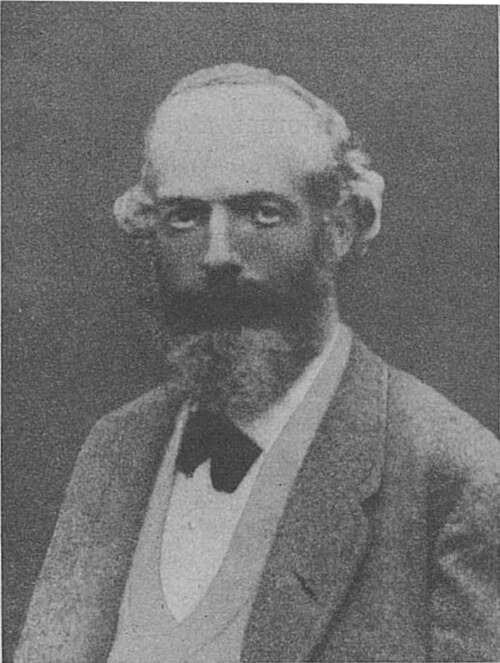
\includegraphics[width=\linewidth]{images/book3/kekule.jpg}
\end{minipage}\hfill
\begin{minipage}[t]{0.74\linewidth}
\vspace{0pt}
في سنة 1865 اقترح أوغست كيكوليه أن ذرات الكربون الست في البنزين تكوّن حلقة
فيها روابط أحادية ومزدوجة متناوبة، ثم بعد ذلك بقليل أن التناوبين
يتبادلان بسرعة كبيرة حتى تتماثل كل الروابط. وقد أعطت الروابط المتساوية التي كشفها حيود
الأشعة السينية، ومدارات $\pi$ الممتدة على الحلقة كلها، حدسَه
صورته الحديثة؛ وفسرت \omterm{thm:b2:huckel:huckel-rule}{قاعدة هوكل}، سنة 1931، لماذا تجعل ستة إلكترونات، لا أربعة ولا
ثمانية، الحلقة متميزة. (صورة شخصية، 1873، مؤلف مجهول، ملكية عامة،
ويكيميديا كومنز.)
\end{minipage}
\end{history}

\section{الترافق والضوء}

\begin{proposition}[فجوة بوليين]\label{prop:b2:huckel:gap}
في بوليين خطي من $n$ كربون ($n$ زوجي)، تكون الفجوة بين أعلى مستوى مشغول
وأدنى مستوى فارغ من مستويات $\pi$ هي $4|\beta|\sin(\pi/(2(n + 1)))$: وهي تتناقص كلما
طالت السلسلة.
\end{proposition}

\begin{proof}
أعلى مستوى مشغول هو $k = n/2$، وأدنى مستوى فارغ $k = n/2 + 1$. ومع $\theta_k =
k\pi/(n + 1)$، $E_{n/2+1} - E_{n/2} = 2|\beta|(\cos\theta_{n/2} - \cos\theta_{n/2+1}) = 4|\beta|
\sin\frac{\theta_{n/2} + \theta_{n/2+1}}{2}\sin\frac{\theta_{n/2+1} - \theta_{n/2}}{2}$، 
والجيب الأول هو $\sin(\pi/2) = 1$. وتتناقص الفجوة مع $n$ لأن $\sin$ متزايدة على
$[0, \pi/2]$.
\end{proof}

\begin{omfigure}
\begin{tikzpicture}
\begin{axis}[width=0.5\linewidth, height=5cm, xmin=0, xmax=22, ymin=0, ymax=2.2,
  axis x line=bottom, axis y line=left, xlabel={\foreignlanguage{arabic}{عدد الكربونات $n$}}, ylabel={\babelsublr{\foreignlanguage{arabic}{الفجوة}$/|\beta|$}},
  tick label style={font=\small}, label style={font=\small}]
\addplot[omThm, thick, mark=*, mark size=1.3pt] table[x=n, y=gap] {figdata/out/bachelor-2-huckel-b.dat};
\end{axis}
\end{tikzpicture}\hfill
\begin{tikzpicture}
\begin{axis}[width=0.48\linewidth, height=5.4cm, xmin=-1, xmax=11, ymin=-2.4, ymax=2.4,
  axis x line=none, axis y line=left, ylabel={$(E - \alpha)/|\beta|$}, clip=false,
  tick label style={font=\small}, label style={font=\small}]
\addplot[only marks, mark=-, mark size=5pt, very thick, omDef] table[x=x, y=e] {figdata/out/bachelor-2-huckel-a.dat};
\draw[densely dotted] (axis cs:-1,0) -- (axis cs:11,0);
\node[anchor=north, font=\scriptsize] at (axis cs:0,-2.45) {C$_2$};
\node[anchor=north, font=\scriptsize] at (axis cs:2,-2.45) {C$_3$};
\node[anchor=north, font=\scriptsize] at (axis cs:4,-2.45) {C$_4$};
\node[anchor=north, font=\scriptsize] at (axis cs:6,-2.45) {C$_6$};
\node[anchor=north, font=\scriptsize] at (axis cs:8,-2.45) {\foreignlanguage{arabic}{حلقة 4}};
\node[anchor=north, font=\scriptsize] at (axis cs:10,-2.45) {\foreignlanguage{arabic}{حلقة 6}};
\end{axis}
\end{tikzpicture}

{\small يمينًا: تتناقص فجوة هوكل للبوليينات الخطية كلما طالت السلسلة، وهذا
سبب امتصاص السلاسل المترافقة الطويلة عند أطوال موجية أطول، حتى المرئي.
يسارًا: المستويات المحسوبة للإيثين والأليل والبوتاديين والهكساتريين (سلاسل) 
وللبوتاديين الحلقي والبنزين (حلقات)؛ والمستويات الرابطة تحت $\alpha$.}
\end{omfigure}

تُدخَل الذرة غير الكربونية بتغيير \omterm{def:b2:diatomic-mos:integrals}{تكامل كولوم} الخاص بها، $\alpha_X = \alpha + h\beta$، 
\omterm{def:b2:diatomic-mos:integrals}{وتكاملات الرنين} لروابطها: وهذا نموذج بوسائط قابلة للضبط، يحفظ
النتائج الكيفية (فالذرة الكهرسلبية، $h > 0$، تجذب كثافة $\pi$ نحو
نفسها) لكن أعداده مُوفَّقة، لا مستنتَجة.

\section{تمارين}

\begin{exercise}[$\star$]\label{exo:b2:huckel:1}
أعطِ $E_\pi$ لكاتيون الأليل وجذره وأنيونه.
\end{exercise}

\begin{exercise}[$\star$]\label{exo:b2:huckel:2}
احسب $E_\pi$ للبوتاديين انطلاقًا من المستويات $\alpha \pm 1.618\beta$، $\alpha \pm 0.618\beta$.
\end{exercise}

\begin{exercise}[$\star$]\label{exo:b2:huckel:3}
\omterm{def:b2:huckel:aromatic}{عطري}، أم \omterm{def:b2:huckel:aromatic}{ضد عطري}، أم لا هذا ولا ذاك (إذا كان مستويًا): البنزين، وأنيون البنتاديينيل الحلقي،
وكاتيون البنتاديينيل الحلقي، وكاتيون التروبيليوم \ce{C7H7+}، والبوتاديين الحلقي، 
والأوكتاتتراين الحلقي المستوي.
\end{exercise}

\begin{exercise}[$\star$]\label{exo:b2:huckel:4}
ارسم دائرة فروست للأوكتاتتراين الحلقي المستوي وضع عليها إلكتروناته $\pi$ الثمانية.
\end{exercise}

\begin{exercise}[$\star\star$]\label{exo:b2:huckel:5}
احسب \omterm{def:b2:huckel:delocalisation}{طاقة اللاتمركز} للبوتاديين وأعطها بوحدة \unit{kJ/mol} مع
$|\beta| = \qty{75}{kJ/mol}$. وقارنها بالقيمة \qty{10}{kJ/mol} المستخلصة من معطيات الهدرجة
للهكسا-1،3-ديين الحلقي.
\end{exercise}

\begin{exercise}[$\star\star$]\label{exo:b2:huckel:6}
احسب مؤشرات روابط $\pi$ للبوتاديين وتنبأ بأي روابطه C--C هي
الأقصر.
\end{exercise}

\begin{exercise}[$\star\star$]\label{exo:b2:huckel:7}
مستويات حلقة خماسية هي $\alpha + 2\beta$، و$\alpha + 0.618\beta$ (مرتين)، 
و$\alpha - 1.618\beta$ (مرتين). املأها لأنيون البنتاديينيل الحلقي ولكاتيونه 
وقارن.
\end{exercise}

\begin{exercise}[$\star\star$]\label{exo:b2:huckel:8}
مستعملًا مستويات حلقة سباعية، فسّر لماذا يسلك بروميد الهبتاترايينيل الحلقي
سلوك ملح، هو بروميد التروبيليوم.
\end{exercise}

\begin{exercise}[$\star\star$]\label{exo:b2:huckel:9}
تحقق من قاعدة الأثر على الهكساتريين، الذي مستوياته $\alpha \pm 1.802\beta$، $\alpha \pm
1.247\beta$، $\alpha \pm 0.445\beta$.
\end{exercise}

\begin{exercise}[$\star\star\star$]\label{exo:b2:huckel:10}
استنتج مستويات الهكساتريين من الصيغة المغلقة، وطاقة لاتمركزه.
\end{exercise}

\begin{exercise}[$\star\star\star$]\label{exo:b2:huckel:11}
كان البوتاديين الحلقي المربع سيملك إلكترونين منفردين. فسّر لماذا يكون الجزيء الحقيقي
مستطيلًا، برابطتين قصيرتين ورابطتين طويلتين.
\end{exercise}

\begin{exercise}[$\star\star\star$]\label{exo:b2:huckel:12}
في نظام $\pi$ ثنائي الذرة \ce{C=X} مع $\alpha_X = \alpha + \beta$ (قيمة نموذجية، $h = 1$) 
و$\beta_{\ce{CX}} = \beta$، أوجد المستويين وشحنتي $\pi$ على C وX من أجل
إلكترونين.
\end{exercise}

\section{مسألة: الطاقة المفقودة في البنزين}

\begin{problem}[{مسألة نهاية الأسبوع --- الاستقرار العطري للبنزين من
أنتالبيات الهدرجة، ومستويات هوكل للبنزين وطاقة لاتمركزه،
وقيمة $|\beta|$، والمقارنة بالهكساتريين 
والأوكتاتتراين الحلقي}]
\label{pb:b2:huckel:1}
المعطيات: أنتالبيات التكوين للغازات (\unit{kJ/mol}): البنزين 82.9،
الهكسا-1،3-ديين الحلقي 104.6، الهكسين الحلقي $-4.3$، الهكسان الحلقي $-123.1$. أطوال الروابط
(pm): البنزين 139.7، الإيثين 133.9، الإيثان 153.6.
% ledger: dfh:C6H6_g, dfh:C6H8_g, dfh:C6H10_g, dfh:C6H12_g, geo:C6H6.rCC, geo:C2H4.rCC, geo:C2H6.rCC

\medskip
\noindent\textbf{الجزء الأول --- الهدرجة.}
\begin{enumerate}
  \item احسب $\Delta_r H^\circ$ لهدرجة الهكسين الحلقي إلى الهكسان الحلقي.
  \item السؤال نفسه للهكسا-1،3-ديين الحلقي.
  \item السؤال نفسه للبنزين.
  \item كم كانت ستطلق ثلاث روابط مزدوجة مستقلة؟
  \item استنتج استقرار البنزين.
  \item قارنه باستقرار الديين المترافق، وعلّق.
\end{enumerate}

\medskip
\noindent\textbf{الجزء الثاني --- البنزين عند هوكل.}
\begin{enumerate}[resume]
  \item اكتب مصفوفة هوكل للبنزين.
  \item أعطِ مستوياته من صيغة الحلقة.
  \item املأها بإلكترونات $\pi$ الستة.
  \item احسب $E_\pi$.
  \item احسب $E_\pi$ لثلاث روابط مزدوجة معزولة.
  \item استنتج \omterm{def:b2:huckel:delocalisation}{طاقة اللاتمركز}.
  \item تحقق من قاعدة الأثر.
\end{enumerate}

\medskip
\noindent\textbf{الجزء الثالث --- قيمة $|\beta|$.}
\begin{enumerate}[resume]
  \item ساوِ \omterm{def:b2:huckel:delocalisation}{طاقة اللاتمركز} بالاستقرار المحسوب في الجزء الأول وأوجد
        $|\beta|$.
  \item بهذه القيمة، تنبأ \omterm{def:b2:huckel:delocalisation}{بطاقة اللاتمركز} للبوتاديين، وقارن
        بالجزء الأول.
  \item احسب مؤشرات روابط $\pi$ للبنزين.
  \item قارنها بمؤشرات روابط البوتاديين.
  \item فسّر لماذا تتساوى أطوال الروابط في البنزين وأين تقع.
\end{enumerate}

\medskip
\noindent\textbf{الجزء الرابع --- حلقات وسلاسل أخرى.}
\begin{enumerate}[resume]
  \item احسب \omterm{def:b2:huckel:delocalisation}{طاقة اللاتمركز} للهكساتريين وقارنها بطاقة البنزين.
  \item أعطِ مستويات الأوكتاتتراين الحلقي المستوي.
  \item املأها بثمانية إلكترونات: ما الخلل؟
  \item كيف يتفادى الجزيء الحقيقي ذلك؟
  \item ما حال البوتاديين الحلقي؟
  \item اذكر \omterm{thm:b2:huckel:huckel-rule}{قاعدة هوكل}.
  \item اذكر قيمة $|\beta|$ التي نحصل عليها بمطابقة \omterm{def:b2:huckel:delocalisation}{طاقة اللاتمركز} للبنزين
        مع استقراره المقيس.
\end{enumerate}
\end{problem}
